%%%%%%%%%%%%%%%%%%%%%%%%%%%%%%%%%%%%%%%%%%%%%%%%%%%%%%%%%%%%%%%%%%%%%%%%%%
%%%%%                         CHAPITRE 7                            %%%%%%
%%%%%%%%%%%%%%%%%%%%%%%%%%%%%%%%%%%%%%%%%%%%%%%%%%%%%%%%%%%%%%%%%%%%%%%%%%

\lhead[\fancyplain{}{\leftmark}]%Pour les pages paires \bfseries
      {\fancyplain{}{}} %Pour les pages impaires
\chead[\fancyplain{}{}]%
      {\fancyplain{}{}}
\rhead[\fancyplain{}{}]%Pour les pages paires 
      {\fancyplain{}{\rightmark}}%Pour les pages impaires \bfseries
\lfoot[\fancyplain{}{}]%
      {\fancyplain{}{}}
\cfoot[\fancyplain{}{\thepage}]%\bfseries
      {\fancyplain{}{\thepage}} %\bfseries
\rfoot[\fancyplain{}{}]%
     {\fancyplain{}{\scriptsize}}


%%%%%%%%%%%%%%%%%%%%%%%%%%%%%%%%%%%%%%%%%%%%%%%%%%%%%%%%%%%%%%%%%%%%%%%%%%
%%%%%                      Start part here                          %%%%%%
%%%%%%%%%%%%%%%%%%%%%%%%%%%%%%%%%%%%%%%%%%%%%%%%%%%%%%%%%%%%%%%%%%%%%%%%%%

\chapter{Capturing equipment along with the athlete - Application to BMX racing}
\label{ch:7}

%==============================================================================	Résumé du chapitre

\begin{center}
\rule{0.7\linewidth}{.5pt}
\begin{minipage}{0.7\linewidth}
\smallskip

\textit{Numerous sports disciplines are practiced with dedicated equipment, which is important to retrieve. However, this equipment can form a closed-loop with the athlete, which makes the task mathematically challenging to resolve. \newline\newline
We analyzed a BMX start sequence, by using OpenPose for 2D human pose estimation, and a custom trained DeepLabCut model for bike detection. We ran Pose2Sim on the joint \{pilot+bike\} 2D estimations, and performed 3D inverse kinematics on a custom OpenSim \{pilot+bike\} model. Expected KPI patterns were successfully measured, however results were inconclusive when constraints were added between the pilot and their equipment. This shows that a 3D markerless analysis of both the athlete and their equipment is possible, which provides additional perspectives for markerless sports motion analysis.\newline\newline
This content has been presented at the "Rencontres scientifiques de la haute performance en cyclisme" \cite{Pagnon2022e}. See Figure~\ref{fig_visabstract5} for a visual abstract.
}

%\smallskip
\end{minipage}
\smallskip
\rule{0.7\linewidth}{.5pt}
\end{center}

\newpage

\minitoc

\vspace*{3cm}

\begin{figure}[hbtp]
	\centering
	\def\svgwidth{1\columnwidth}
	\fontsize{10pt}{10pt}\selectfont
	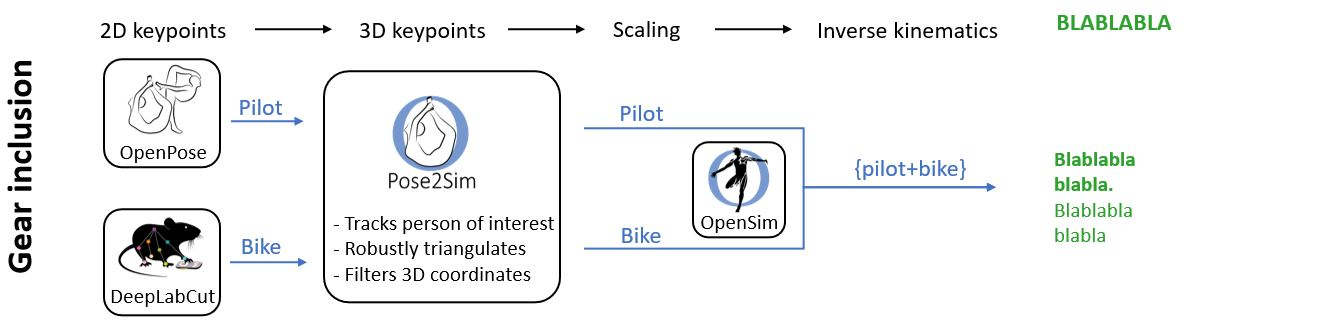
\includegraphics[width=\linewidth]{"../Intro/Figures/Fig_VisAbstract5.JPG"}
      \caption{Visual abstract for joint analysis of the athlete with OpenPose, and their equipment with DeepLabCut.}
	\label{fig_visabstract5}
\end{figure}

\newpage


\section{Introduction}
\subsection{The importance of equipment}

Numerous sports disciplines involve equipment; and sometimes, the motion of this equipment and of the athlete are of equal importance. Tracking a ball in soccer can help understand anticipated actions and game dynamics \cite{Ghasemzadeh2021}, documenting the motion of a tennis racket \cite{Martin2013}, a hockey stick \cite{Kays2017} or oars of a rowing boat \cite{Ruffaldi2015} gives insight on the interactions between the athlete and their gear, and retrieving information about skis \cite{Ludwig2020} or bike parts \cite{Rosenhahn2008} can help quantify specific posture cues.

However, this is challenging on several levels. First, the equipment needs to be tracked. This is straightforward with marker-based or IMU based technologies: one can simply equip the object with an additional marker, or sensor. However, this is more complicated with a markerless approach based on deep-learning, as it involves labelling each point or object of interest on numerous images, and training a specific model. Second, in case the equipment is multisegmented, its own kinematics needs to be calculated, either with a 6DoF approach, or via inverse kinematics. In the latter case, a specific model needs to be crafted, with accurate joint specifications and segment dimensions. Third, when the athlete is in contact with their equipment, it can be interesting to solve the combined kinematics of the whole $\{athlete+equipment\}$ system. The problem remains simple if the kinematic chain remains open like in a tennis serve \cite{Martin2013}, however when the equipment makes it a closed loop, this can become rapidly much more complex, and unsolvable. The privileged solution consists in "breaking" the kinematic chain to treat it as an open loop. The broken joints can then optionally be reassembled using constraints, which has been reported to significantly improve accuracy \cite{Rosenhahn2008,Fohanno2014}.

BMX race represents such a problem. Coaches are interested in the motion of the bike as regards to the athlete. As a consequence, the bike needs to be tracked, modeled, and then its kinematics needs to be computed. This is especially difficult, because both feet and both hands are in contact with the bike, which makes it a particularly constrained closed chain, hence very difficult to solve. 


\subsection{The start in BMX racing}
BMX race differs from other cycling disciplines in several ways, one of them being the short duration and of the effort. At the elite level, each race lasts about 30 to 40 seconds \cite{Cowell2012}. Hence, the winner is the one who has not only averaged the greatest speed, but also taken the shortest trajectory. In order to be able to choose the best one without being obstructed by other riders, one has to take a good start. \cite{Rylands2014} analyzed the statistics of 348 elite racers in UCI (Union cyclist international) competitions, and found a strong correlation between early placing and final placing. Most authors actually study the start, rather than any other part of the race \cite{Zabala2009,Gianikellis2011,Chiementin2012,Kalichova2013,Rylands2014}.

Moreover, riders never sit on their saddle. When cycling off the saddle in road cycling, arms have been shown to be more involved since they push and pull the handlebar \cite{Stone1993}, as the body is brought upward and forward over the axis of crank rotation. Hence, this discipline requires conducting whole body analysis. \cite{Gianikellis2011} suggest that for a faster start, the Range Of Motion (ROM) of the knee needs to be smaller than that of the trunk. \cite{Kalichova2013} finds a clear asymmetry in upper-body motion, both in terms of elbow and shoulder joint angles. However, as these two are case studies, it is hard to give much trust to these measurements in terms of performance. More specifically, the first movement initiated during a BMX start is the so-called "slingshot" maneuver. It consists in moving the body down and forward, while the bike goes in the opposite direction, the front wheel lifting noticeably. This plyometric countermovement occurs before the first pedal stroke, and before the gate has entirely dropped. According to \cite{Gross2017}, this technique is highly effective. It involves a stretch-shortening cycle of the front knee, and the counter-movement is more pronounced and initiated earlier in better riders. This confirms that the complex motion of the bike as regards to the pilot at start is of crucial importance (see Figure~\ref{fig_bmxstart}). 

\cite{Grigg2017} concludes her literature review by underlying that research associating kinematic characteristics and gate start performance would be useful for coaches. She also adds that both equipment and rider analysis are of critical importance. Finally, she points out that research should be done on-field, rather than in lab conditions which would introduce bias. As a consequence, we captured the start in BMX race, in ecologically valid conditions, tracking both the pilot and the bike movement in 3 dimensions, with and without closed-loop constraints, with a markerless protocol. The goal was to propose a method for such an objective, and verify whether some kinematic variables could be measured.

\begin{figure}[hbtp]
	\centering
	\def\svgwidth{1\columnwidth}
	\fontsize{10pt}{10pt}\selectfont
	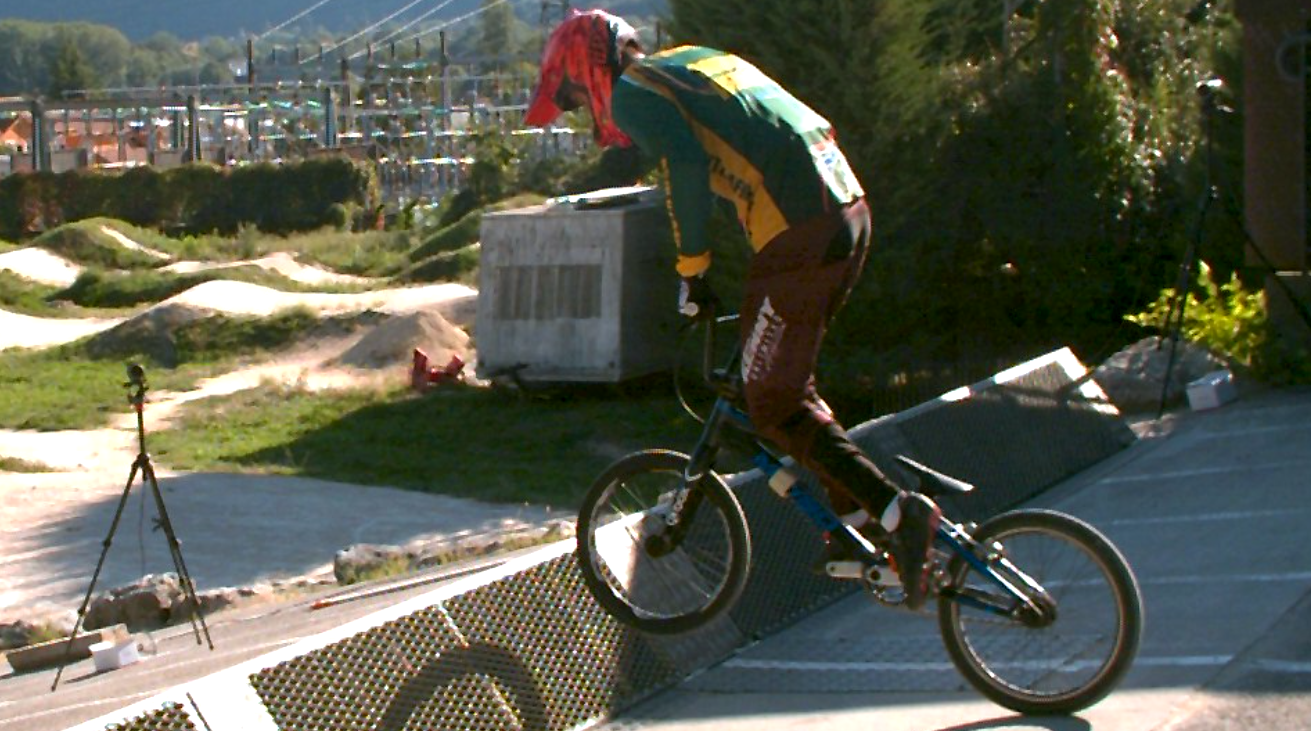
\includegraphics[width=\linewidth]{"../Chap7/Figures/BMXStart.PNG"}
	\caption{The early slingshot maneuver in BMX race.}
	\label{fig_bmxstart}
\end{figure}


\section{Methods}

\subsection{Material and protocol}
As this was a preliminary experiment, we conducted this study on one single pilot, and examined one single start. Only 6 Qualisys Miqus cameras were used. The resolution was only of 1 megapixel, however the framerate was of 120 fps. Synchronization was achieved with a hardware trigger, but calibration was not successful with the standard method using a wand equipped with markers. In broad daylight, markers were either missing, or confused with artifact reflections. Hence, we calibrated on the grid dimensions, in the same way as described in previous chapter (see \nameref{calib_pnp}). 

The amateur pilot involved in this study signed a form of informed consent. He was first captured standing on a T-pose for scaling the skeletal OpenSim model accordingly, and then performed 3 starts in conditions similar to those of a competition. He was accustomed to the BMX track and the 5 meters starting hill, as well as with the standard gate and sound signal used for setting off the start. He wore his usual equipment, and confirmed that his movement and concentration were not hindered by the capture. Among the 3 starts the pilot executed, only one of them was studied. 


\subsection{Pilot inverse kinematics}
The pilot was detected, triangulated, scaled on a T-pose, and his kinematics was computed with the default Pose2Sim parameters \cite{Pagnon2022b}. 


\subsection{Bike inverse kinematics}
OpenPose models only detect human beings, and up to our knowledge, there is no existing deep-learning based model for tracking a BMX bike. Several options were available: segmenting the bike in 2D, and reconstructing its shape, but it would have been difficult to rendered its handle, crank, pedals, and wheels movements. Hand labelling videos with \cite{Kinovea}, and tracking these points on the rest of the video is one common approach \cite{Grigg2018}, but the tracking tends to be lost when occlusions happen, and this is not scalable: the initial labelling has to be done again for each new video and each new point of view. Another option is to train our own deep-learning model.

DeepLabCut \cite{Mathis2018, Lauer2022} is a toolbox originally made to train custom models for animal keypoint recognition, which leverages transfer learning to achieve good results with minimal training data. We used it to label 9 keypoints on a BMX bike, enough to be able to correctly scale the model and to render its internal motion (see Figure~\ref{fig_bikemodel}). We labeled 210 images extracted from our videos and from videos found on YouTube, with varying perspectives, image qualities, and number of bikes on the frame. We trained DeepLabut in multiAnimal mode, which has been reported to be more complex to use and to take longer training time, but to produce more accurate results in challenging conditions. Network architecture and augmentation methods were left to default. Loss reached a plateau after 110,000 iterations, at which point we stopped the training procedure. Default Pose2Sim parameters were used for tracking, weighted triangulation, and filtering of the bike coordinates. 

\begin{figure}[hbtp]
	\centering
	\def\svgwidth{1\columnwidth}
	\fontsize{10pt}{10pt}\selectfont
	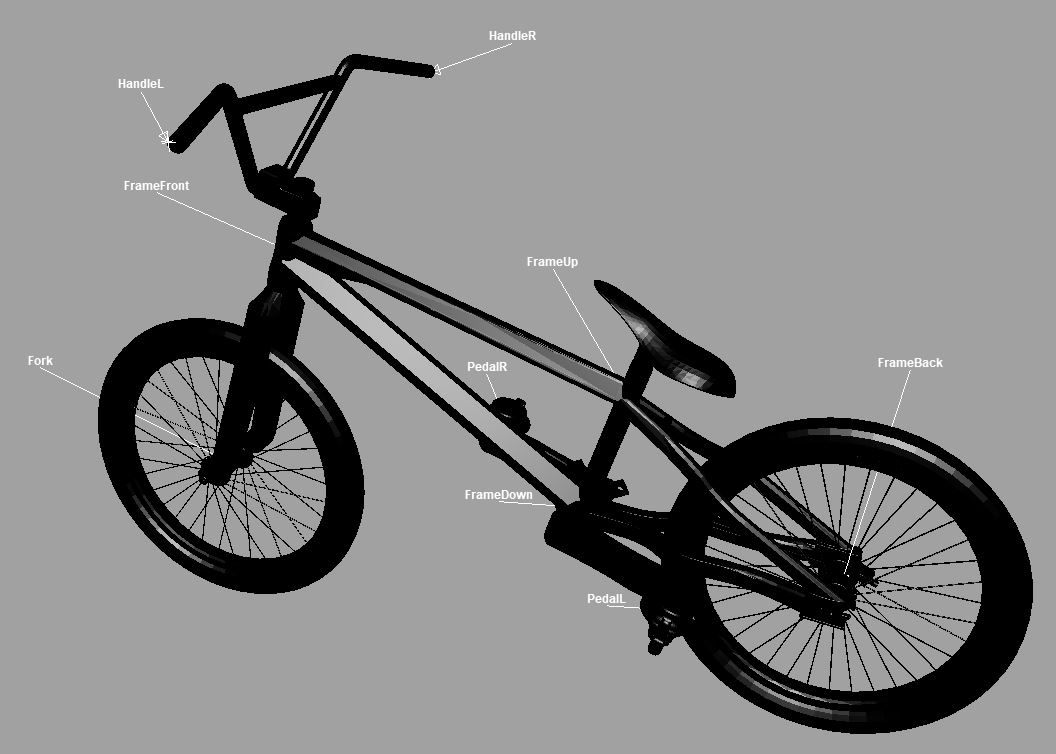
\includegraphics[width=\linewidth]{"../Chap7/Figures/Bike_keypoints.PNG"}
	\caption{The articulated bike model, and the labels DeepLabCut was trained to recognize.}
	\label{fig_bikemodel}
\end{figure}

An articulated BMX bike model was designed on SolidWorks, and although we don't need for kinematics, its inertial properties were validated against a real bike. Pin joints modeled the articulations between the fork and the frame, the frame and each wheel, the frame and the crankset, and the crankset and each pedal (see Figure~\ref{fig_bikemodel}). The frame, the handlebar, and the crankset were each scaled according to 3D keypoint pairs, uniformly along the 3 space dimensions. Marker weights were all set to 1 for inverse kinematics. 


\subsection{Joined pilot and bike inverse kinematics}
The pilot and the bike form a kinematic chain which is closed in multiple places, due to contacts between feet and pedals, and hands and handlebar. Such a chain is not solvable, hence it needs to be "broken". There are several ways to do it: the most obvious one consists in modeling contact not with joints, but with constraints. OpenSim available constraints Weld, Point, or coordinate coupler. Weld constraints are not appropriate, since in reality, both hands and feet can rotate around pedals and handlebar. Point constraints are not appropriate either, since the pilot can translate their hands along the handlebar. Moreover, pedals may not be detected perfectly, so it is important that feet have more latitude. Coordinate coupler implies that there is a relation between coordinates, e.g., between the rotation of hands and the rotation of the handlebar. This is not the case. Moreover, soft constraints are not embedded in OpenSim. 

As constraints cannot be too tight, we took a slightly different approach. We duplicated hands and feet, one version attached to the pilot, and the other to the bike. The two versions were welded together. However, the one connected to the bike could be articulated with any kind of joint, with as many degrees of freedom as needed, and with joint limits as loose or as tight as needed (See Figure~\ref{fig_bikepilotchain}). 

\begin{figure}[hbtp]
	\centering
	\def\svgwidth{1\columnwidth}
	\fontsize{10pt}{10pt}\selectfont
	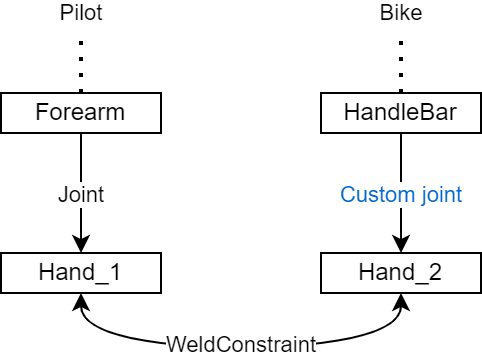
\includegraphics[width=0.4\linewidth]{"../Chap7/Figures/bikepilotChain.png"}
	\caption{The trick used to break the kinematic chain, and constrain it while keeping more degrees of freedom than OpenSim allows. Any custom joint could be used (e.g., a cylindrical joint), and joint limits could be adjusted.}
	\label{fig_bikepilotchain}
\end{figure}

We scaled both pilot and bike independently, by disabling constraints. We then conducted inverse kinematic analysis of both pilot and bike, in two conditions: first, without enabling constraints. Then, with enabling them and comparing the effects of several kinds of joints between hands and handlebar, and feet and pedals: ball joints (all rotations allowed), cylindrical joints (rotation and translation permitted along the handlebar axis), free joints (all rotations and translations allowed). Joint translations were limited to 20 cm. Weights were taken identical to those previously reported, both for scaling and inverse kinematics. 


\subsection{Performance indicators assessment}
We investigated a wide variety of the key performance indicators reported in the literature. On the pilot, the flexion of the front knee, which should show a plyometric action, and the flexion of both shoulders, which should be asymmetric. On the bike, the elevation of the front wheel, and the angle of the handlebar. On pilot and bike together, we investigated the forward speed of the center of motion (COM) of the bike, and of the pilot, which should point in different directions during the slingshot maneuver. We also reported the rotational excursion of the right foot and right pedal around the center of the crankset, which should be similar since in reality, they are attached together. All results were filtered with a zero-lag fourth order 10 Hz low-pass Butterworth filter.


\section{Results}
\subsection{Inverse kinematics with and without constraints}
Calibration was not as accurate as it would have been with a gold-standard method, but it remains in the centimetric order of magnitude. Synchronization was triggered by hardware, and thus perfect. However, low number of cameras, low image resolution, low contrast, and strong occlusions lead to 2D pose estimations of relatively poor quality, both for the pilot detected with OpenPose, and for the bike detected with DeepLabCut (up to 10 px error between estimations and labels for the latter, which corresponds to about 3.5 cm). This was especially true in the foot region, which was subjected to jittering. Results were not much improved by changing OpenPose model, modifying Pose2Sim triangulation and filtering parameters, and adjusting OpenSim scaling and inverse kinematics weights, neither for the pilot nor for the bike. Consequently, we used default parameters. 

Constraining both pilot and bike OpenSim models together was proven unsuccessful for the most part, regardless of the type of custom joint used, even with all degrees of freedom allowed (with joint limits). Using point constraints instead of weld ones between both sets of hands and of feet did not make a difference. Increasing assembly error tolerance was also proven unsuccessful. The only way OpenSim inverse kinematics could converge with constraints was if only feet were constrained, and hands were free. However, no comparative analysis has been done to assess whether results were better than when disabling all constraints.

We had previously captured similar BMX start data, with a higher quality marker-based approach. Conducting the same analysis on these data was mostly unsuccessful too. We tried using only joint markers, or the full set, with similar outcome. %This suggests that not only the quality of our markerless data is at fault, but mostly, the model is overconstrained.

\begin{figure}[hbtp]
	\centering
	\def\svgwidth{1\columnwidth}
	\fontsize{10pt}{10pt}\selectfont
	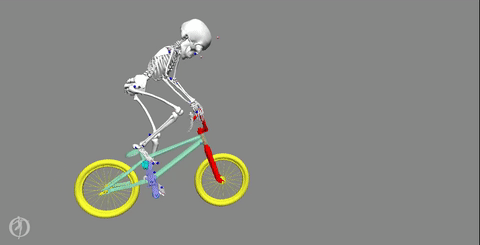
\includegraphics[width=\linewidth]{"../Chap7/Figures/BMXPilot.png"}
	\caption{OpenSim inverse kinematics was successful when no constraints were applied between the BMX pilot and bike. Note that the feet and hands are jittering due to the low number of cameras and to occlusions, which could be improved if constraints were applied between feet and pedals, and hands and handle. See animated version \href{https://github.com/perfanalytics/pose2sim/blob/main/Content/Activities_verylow.gif}{here}.}
	\label{fig_bmxpilot}
\end{figure}
% \begin{frame}{Embedded Animation}
%   \animategraphics[loop,controls,width=0.7\linewidth]{25}{"../Chap7/Figures/bmxgif/bmx"}{1}{180}
% \end{frame}


\FloatBarrier
\subsection{Key performance indicators}

Concerning the pilot, one can notice a flexion, then extension of the (left) front knee, which indicates a plyometric movement during the slingshot phase. Shoulder flexion of both arms present relatively similar waveforms, although the right one is slightly more flexed all along the maneuver, which is consistent with the fact that the body needs to pivot to the right in order to push to the maximum on the left pedal. The elevation of the front wheel is very noticeable. However, the handlebar rotation is not very coherent: in fact, due to bad estimations, the handlebar does a complete spin before recovering a consistent angle. The forward speed of the COM of the pilot is noisy, but it shows that it increases linearly during the slingshot phase. Conversely, the speed of the bike first points backward before pointing quickly forward, until it balances out with the pilot speed. The rotational excursion of the right foot is similar to the one of the pedal, but it is more noisy. 

\begin{figure}[hbtp]
	\centering
	\def\svgwidth{1\columnwidth}
	\fontsize{10pt}{10pt}\selectfont
	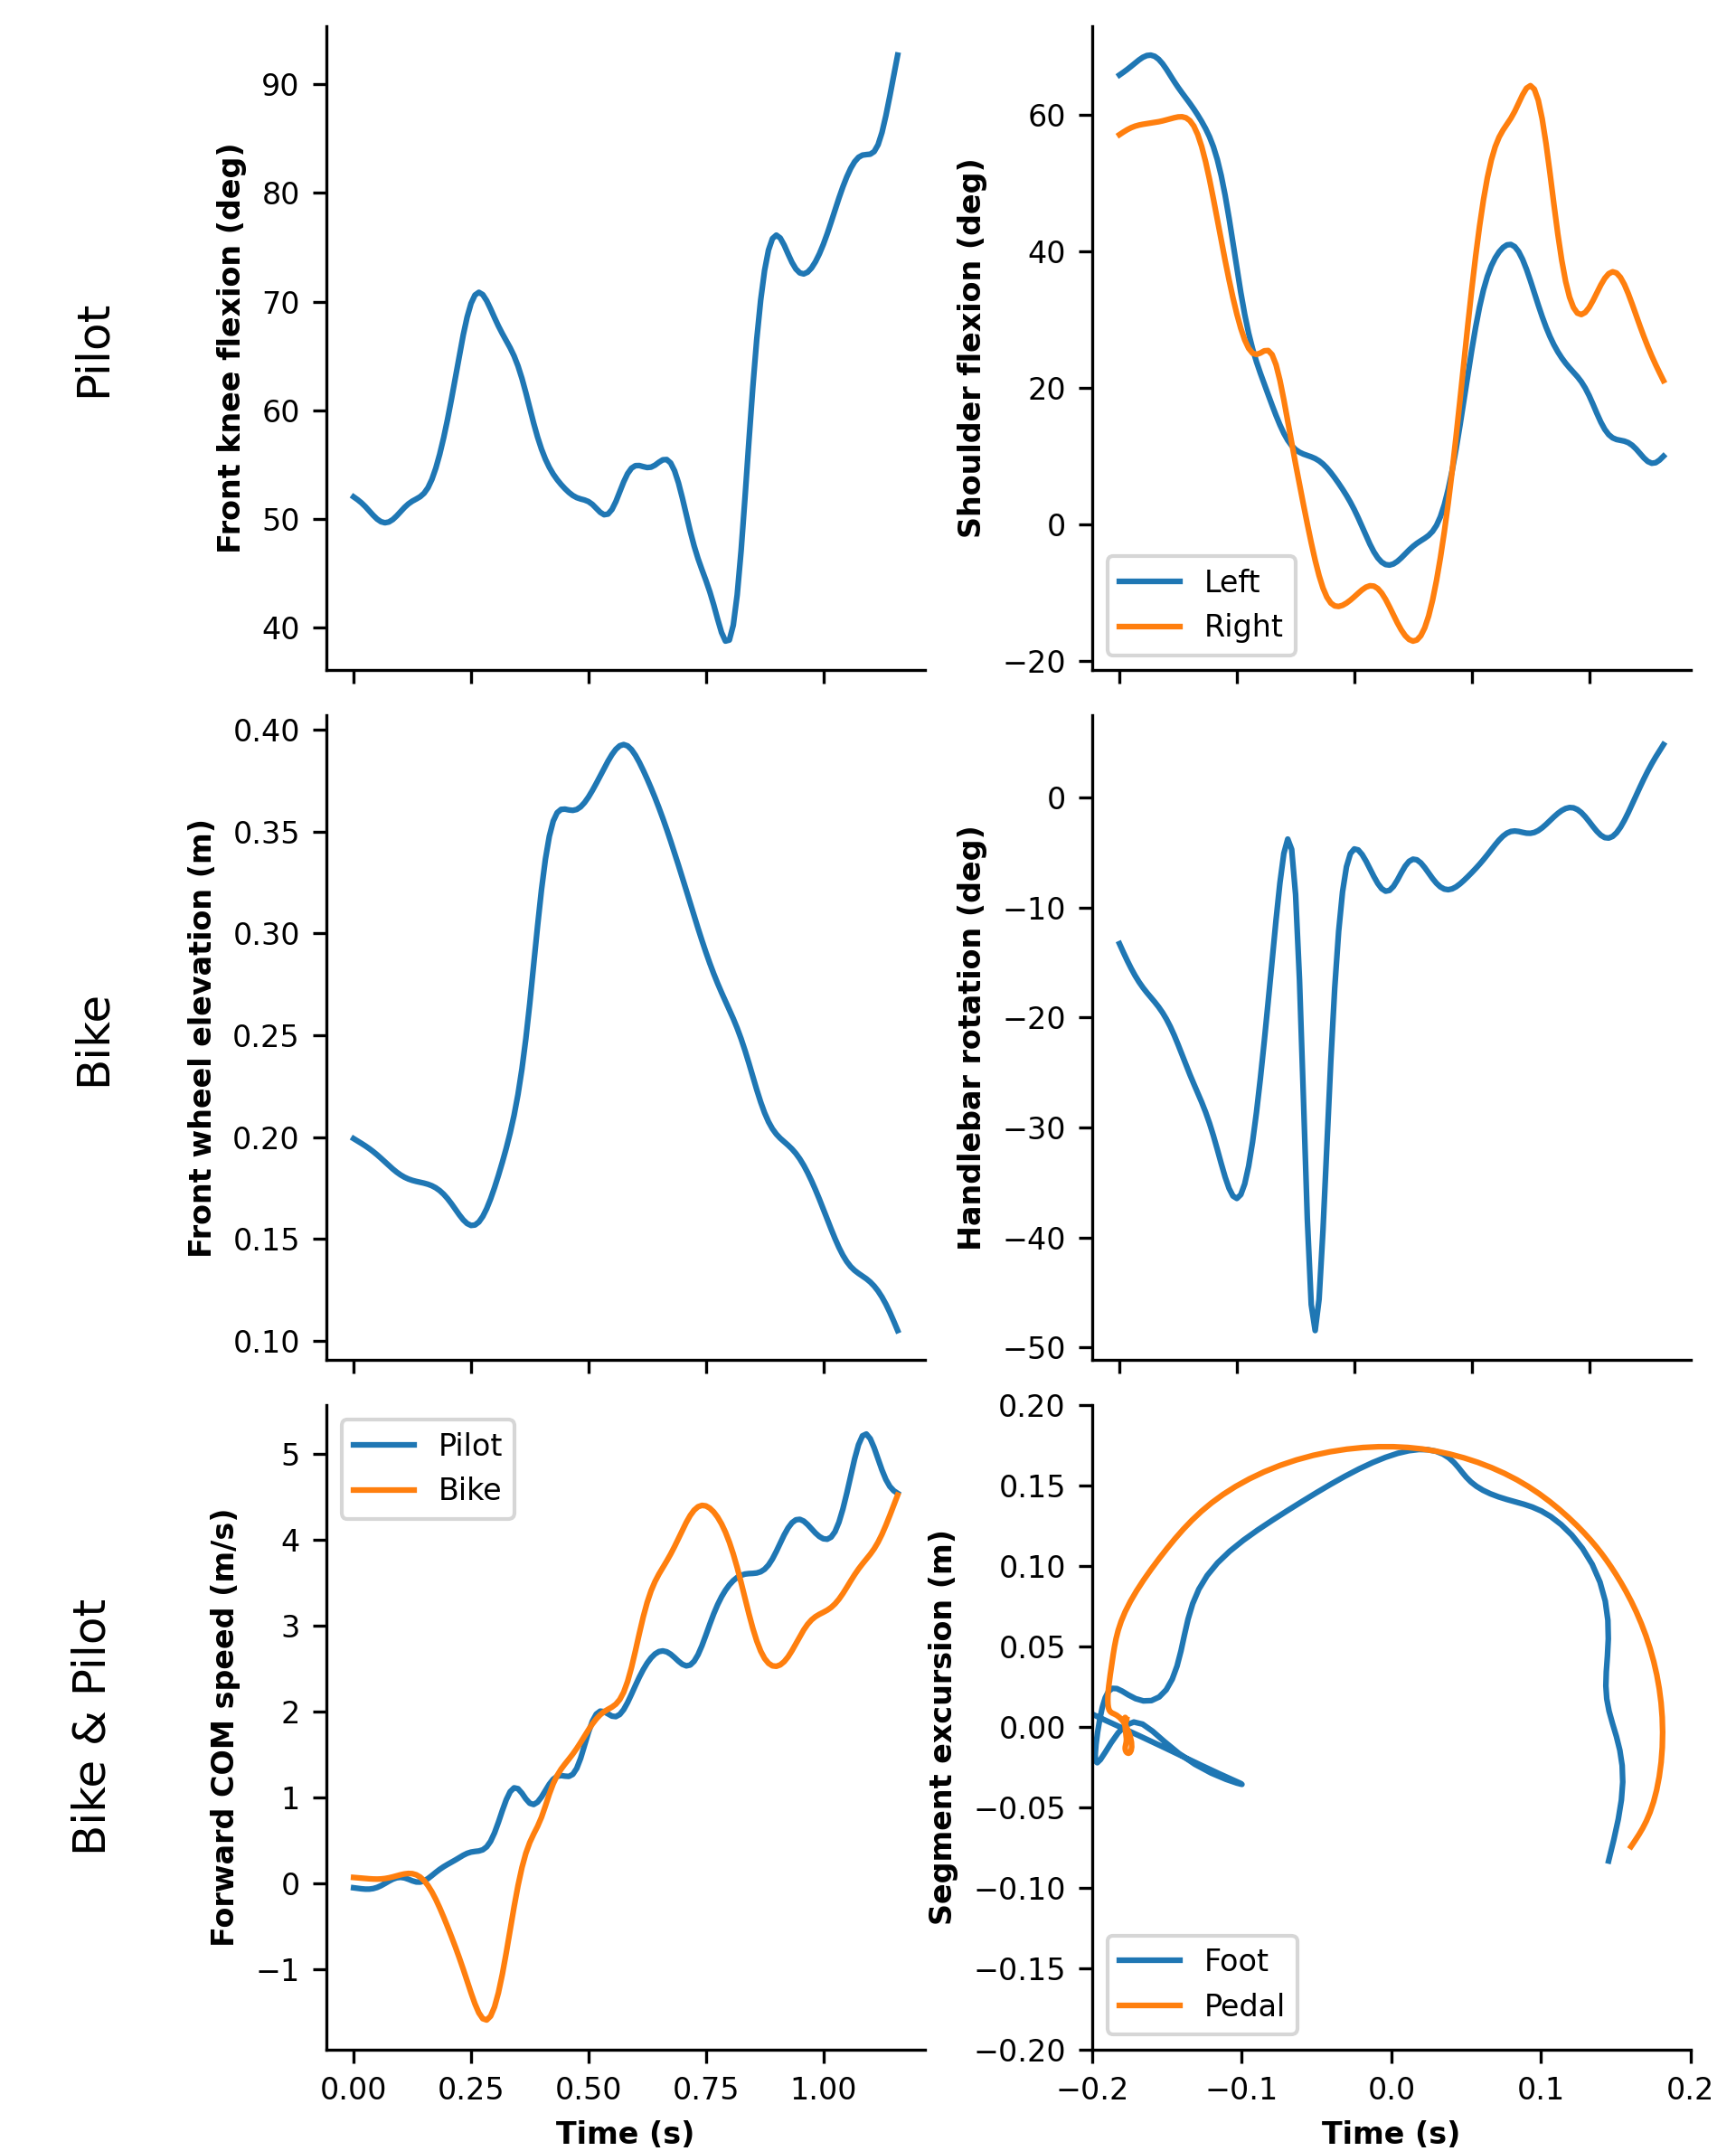
\includegraphics[width=0.85\linewidth, left]{"../Chap7/Figures/KPIs_BMX.png"}
	\caption{Some key performance indicators of the BMX slingshot phase captured with a markerless protocol.}
	\label{fig_kpisbmx}
\end{figure}


\FloatBarrier
\section{Discussion}
\subsection{Kinematic analysis of the athlete with their equipment}
The objective of this preliminary study was to verify whether an athlete could be detected with their equipment with a 3D markerless protocol, in ecologically valid conditions. BMX race involves such a problem, where detecting both a pilot and their bike can bring out important information. Performing the kinematic analysis of a BMX bike involves training a deep-learning model with DeepLabCut to detect 2D bike keypoint, and then creating an OpenSim "skeletal" bike model, with coherent geometry and joints between parts. This is especially challenging to carry out, because a bike is multi-articulated, and it forms several closed loops with the pilot. Hence, one needs to find a way to break the kinematic chain in 4 different places, and then to constrain it together in a coherent and computable way.

As it is decisive in a race, the slingshot phase of the start was analyzed, and a wide variety of pertinent key performance indicators was investigated, targeting pilot, bike, and pilot and bike together. Since only one trial was analyzed, no accuracy assessment was possible. However, we could verify whether expected patterns were observed. When not constraints were imposed between the pilot and the bike, the plyometric movement of the front knee was detectable, and the difference between left and right shoulder flexion, too. The elevation of the front wheel was clearly visible, however an implausible spin of the handlebar was reported. The "slingshot" movement of the bike could also be detected, and we noticed that on the opposite, the pilot COM speed increased linearly. The foot motion was in accordance with the rotation of the pedal, however it was more noisy. Overall, performing 3D markerless inverse kinematics of both a BMX pilot and their bike, and \emph{a fortiori}, of an athlete and their equipment, seems possible.


\subsection{Inverse kinematics in closed loop}
One can assume that if the handledbar were constrained to correctly detected hands, it would not suffer from this abnormal spin; and that if feet were constrained to the pedals, their excursion would be less noisy. However, inverse kinematics did not converge when implementing constraints. This can be attributed to two main reasons: first, the poor quality of our detections, and second, the overly constrained kinematic chain. 

Gold-standard calibration was unsuccessful, and we resorted to a less accurate post-calibration procedure, whose extrinsic parameters were determined by the dimensions of the starting grid. In order to reach high framerate, we lowered the resolution of the videos, which made the detection less precise. Finally, using only 6 cameras was not sufficient considering such a low contrast, and such strong occlusions from the pilot, their bike, and the gate start. This was especially obvious for the feet and the front wheel, hidden before before the gate dropped. However, despite the use of few training data, the DeepLabCut bike model did not seem to perform more poorly than the OpenPose human one. Moreover, conducting a similar study with high quality marker-based data was not successful either, which suggests that the quality of our markerless data is not the only parameter at fault. 

Ultimately, the model is most likely overconstrained. Solutions regarding this issue remain unclear. Better data, with higher resolution, higher number of cameras, and better calibration, is the first element to improve, which is probably necessary but not sufficient. Pilot and bike are both composed of rigid bodies, and constraining them together may have lead to some geometric incompatibilities, even after scaling. For instance, the angle between the fork and the bike frame might be different between the bike model and the one used by the pilot. Liberating some degrees of freedom did not seem to make any difference, however disabling some of the constraints (e.g., hand constraints) allowed inverse kinematics to work. Since the handlebar is constrained to the hands, its weights don't need to be as high; similarly, the weights of pedals could be lowered in order not to impose any incompatible conditions for the inverse kinematics solver. Alternatively, one could look into other inverse kinematic algorithms, e.g., some which would allow using soft constraints instead of hard ones \cite{Fohanno2014}.


\subsection{Conclusion}
These results show that a 3D markerless analysis of both the athlete and their equipment is possible, which provides additional perspectives for markerless sports motion analysis. However, this was only a preliminary experiment, and several elements should be improved before drawing any definitive conclusion. First, more cameras with better definition should be used. This is especially important if a larger field of view has to be captured, e.g., if a longer portion of the track would need to be investigated. Action cameras meet such requirements, and they offer the additional advantages of being light and wireless. However, they need post calibration and post-synchronization, but this has been proven feasible (See Chapter~\ref{ch:6}). Second, in case the equipment forms a closed-loop with the athlete, results are not conclusive yet. Hence, more work needs to be done to understand how connections between the equipment and the athlete can be taken into account, without preventing inverse kinematics to converge.

Such a protocol can be applied to any individual sport. When some equipment needs to be detected, two additional steps have to be completed. First, the training of a deep-learning model, which can be done relatively seamlessly and with little image labelling, thanks to transfer learning leveraged by DeepLabCut. Second, if only inverse kinematics is desired, designing an OpenSim model is also relatively easy, as only a few segment dimensions and joint properties are needed, without any consideration for inertial properties. Both steps are scalable, and need to be performed only once for all individuals, environments, and camera properties and positioning. 

% Kalman smoothing? 

% Bushing forces? % Alternatively, you could attach the toes and/or hands to the bike via BushingForces (or sprint forces ?) (https://simtk.org/api_docs/opensim/api_docs/classOpenSim_1_1BushingForce.html#details).





% Rosenhahn2008 snowboard: closed kinematic chain: pas évident, voir [17] ( reduced equations of robotic systems using Lie groups). Eux: soft constraints (invariances -> numeric) rather than joints (analytic)
% Formalisme joint vs constraint Part 3.1 https://sci-hub.se/https://ieeexplore.ieee.org/document/4587520




% riders use a very particular technique for gaining speed in the bumps without pedaling, known as “pumping” 
% [Cowell 2012, Rylands 2016]: on the way up they decrease their loss in gravitational potential energy by bending their arms and legs, and on the way down they increase their kinetic energy by extending their limbs. Finally, athletes have to take big jumps and to operate sharp turns without colliding with each other. Unfortunately, according to [Novak & Dascombe 2014] the majority of performance characteristics studies have been conducted on road cycling athletes.  [Cowell 2012] shows that hip and knee extensors, as well as horizontal shoulder abductors and adductors are heavily relied upon all along the race. 